\section{Results}
\label{sec:Chapter3} \index{Chapter3}

\subsection{Постановка основных экспериментов}
В качестве основной модели для проведения численных экспериментов выбрана архитектура из $N = 4$ ридберговских атомов, расположенных в узлах квадратной решётки. Временная зависимость параметров гаильтониана, описанная в пункте \ref{seq:simulation}, разбивалась на $\text{num\_time\_segments} = 5$ сегментов. Данная конфигурация является приемлемым компромиссом между выразительностью модели и вычислительными затратами на симуляцию её динамики.

На выходе квантовой сети производилось измерение одно- и двухкубитных наблюдаемых Паули ($Z_i$ и $Z_i Z_j$). Полученные значения подавались на обучаемый линейный слой для отображения в пространство признаков, соответствующее числу классов решаемой задачи. В такой постановке для задачи бинарной классификации общее число обучаемых параметров модели составило $103$.

\begin{figure}[h!]
    \centering
    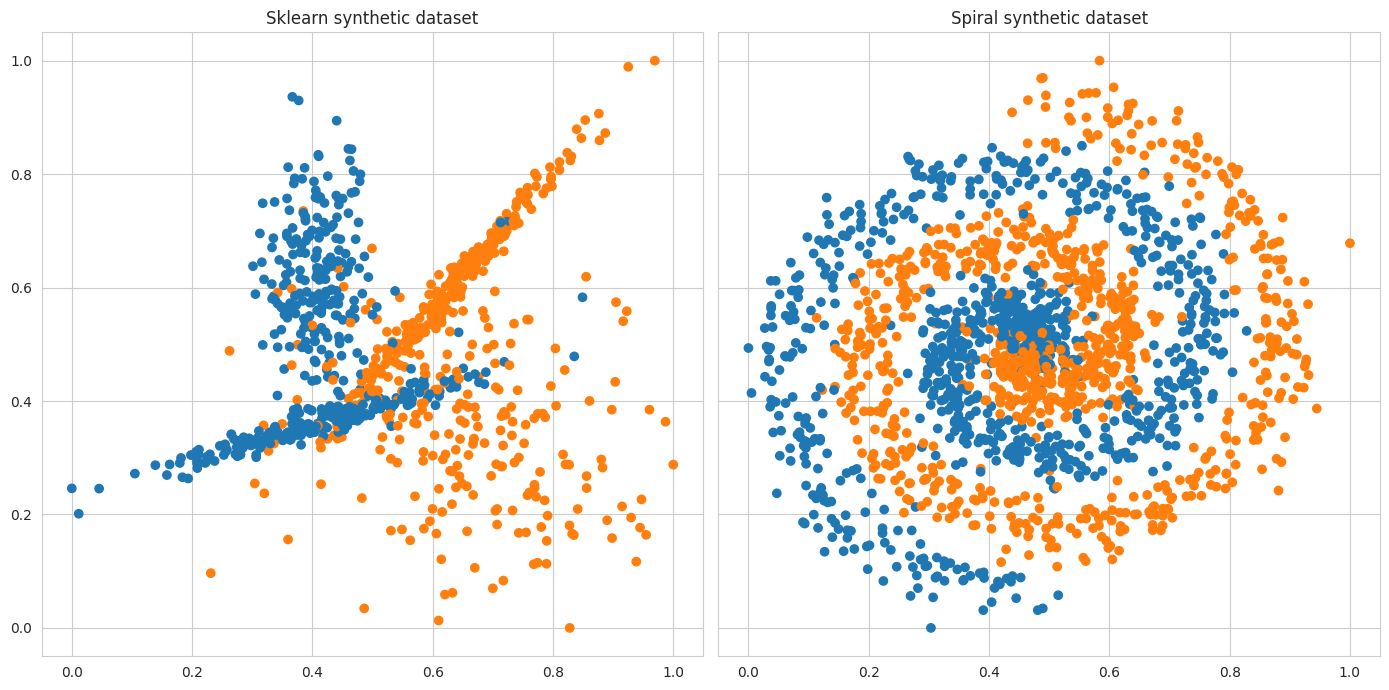
\includegraphics[width=1\linewidth]{images/datasets.png}
    \caption{Синтетические датасеты для обучения. \textbf{Слева:} многомерная классификация (сгенерирована функцией \texttt{make\_classification}). На графике приведен двумерный вариант для визуализации; в основных экспериментах использовалось 4 признака. \textbf{Справа:} Зашумлённый спиральный датасет, который служит для проверки экспрессивности квантовой модели.}
    \label{fig:datasets}
\end{figure}

В предлагаемом подходе входные признаки распределяются по схеме «один признак на один атом». Учитывая высокую вычислительную сложность рассчёта прямого и обратного подхода по квантовой сети, для обучения были выбраны два компактных синтетических набора данных. Все входные значения были отнормированы в диапазон $[0, 1]$. Визуализация тренировочных данных представлена на Рисунке \ref{fig:datasets}.

Выбор и конфигурация датасетов обусловлены необходимостью строгого разделения классического и квантового вклада в итоговый результат:
\begin{enumerate}
    \item \textbf{Многомерная классификация (4 признака):} сгенерирован с помощью функции \texttt{make\_classification} (библиотека scikit-learn). Использовалась конфигурация с 4 признаками и 2 кластерами на класс. Это позволило реализовать прямую передачу данных в квантовый слой без использования промежуточного классического линейного слоя, изменяющего размерность. Такой подход является методологически важным: поскольку задача потенциально допускает достижение приемлемой точности даже линейными методами, исключение обучаемого препроцессинга позволяет изолированно измерить влияние квантовой архитектуры на качество классификации.
    \item \textbf{Спиральный датасет (2 признака):} сгенерирован для оценки экспрессивности предложенной архитектуры при решении существенно нелинейных задач. В этой постановке использовался минимальный линейный слой для отображения двух входных признаков на четыре атома системы. Важно отметить, что в силу топологии <<спирали>>, линейное преобразование само по себе не способно упростить задачу классификации. Таким образом, высокая точность, достигнутая на данном датасете, может быть интерпретирована как доказательство нетривиальности работы квантового слоя.
\end{enumerate}

Подбор гиперпараметров (начальные длительности импульсов, амплитуды, межатомное расстояние и скорость обучения) осуществлялся с использованием байесовской оптимизации (библиотека Optuna). Для каждого набора данных было проведено 400 итераций поиска (trials) длительностью по 500 эпох каждая. Пределы learning\_rate были выставлены так, что за такое число эпох любой запуск сходился.

В качестве бейзлайна была выбрана архитектура MLP с одним скрытым слоем. Размер скрытого слоя подбирался таким образом, чтобы число тренируемых параметров MLP совпадало с квантовой архитектурой.

\subsection{Анализ графиков обучения}

На Рисунке \ref{fig:training_curves} представлены результаты обучения разных конфигураций модели на двух датасетах. Сравнительный анализ графиков позволяет сделать следующие выводы:
\begin{itemize}
    \item \textbf{Экспрессивность.} На спиральном наборе данных (Рисунок \ref{fig:results_spiral}) наблюдается ярко выраженное преимущество: в то время как классический MLP-бейзлайн с эквивалентным числом параметров демонстрирует не способность решить задачу, квантовая модель достигает практически идеальной классификации.
    \item \textbf{Роль квантовой запутанности.}Абляционное исследование выявило критическую важность взаимодействия между атомами. В режиме «disentangled» (искусственное выключение взаимодействия в гамильтониане) и при исключении двухкубитных корреляторов из измерений наблюдается заметная деградация модели. Это доказывает, что квантовая запутанность вносит существенный вклад в работоспособность предложенной архитектуры.
    \item \textbf{Численная устойчивость.} Для всех конфигураций модели на основе ридберговских атомов характерны сильные флуктуации кривых обучения. Это обусловлено высокой чувствительностью функции потерь к параметрам лазерных импульсов в окрестности ридберговской блокады. Несмотря на это, повторяющаяся тенденция к уменьшению тренировочного лосса подтверждает робастность обучения предложенной архитектуры.
\end{itemize}

\subsection{Анализ гиперпараметров}

\begin{figure}[h!]
    \centering
    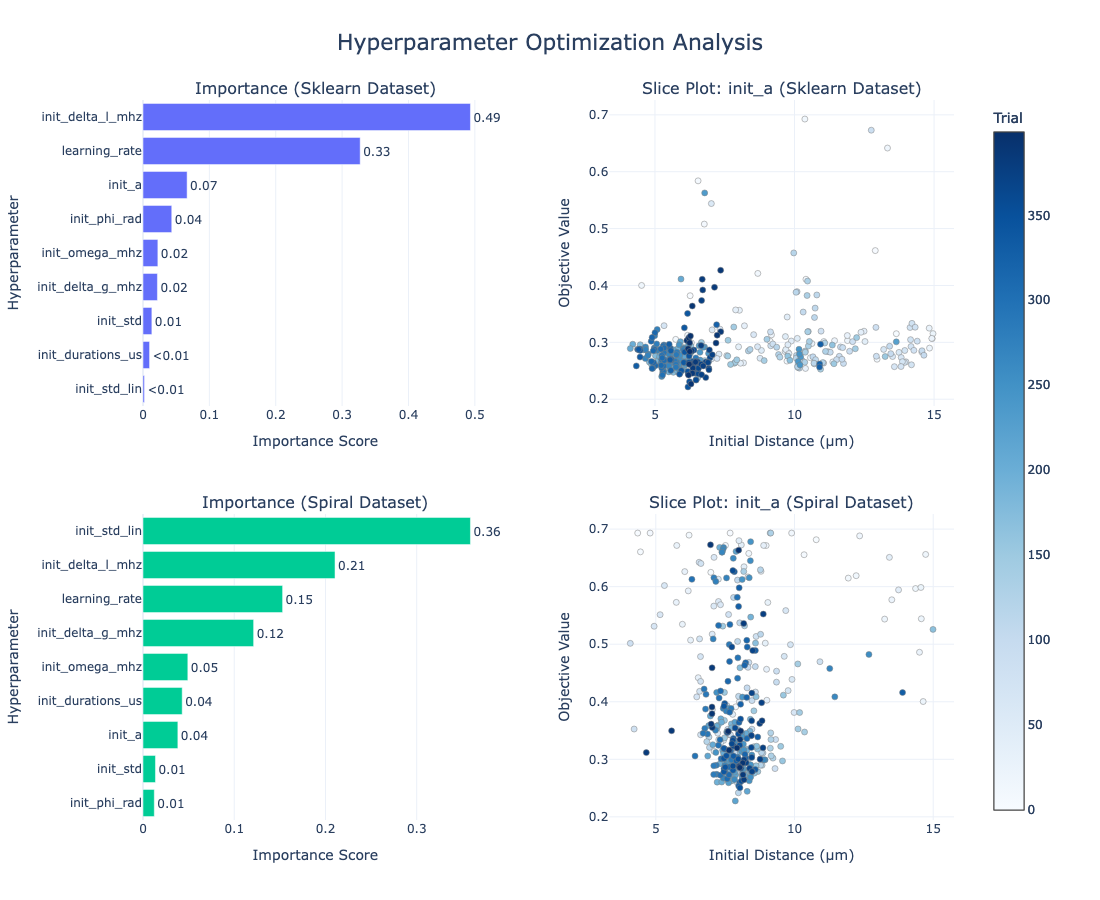
\includegraphics[width=0.8\linewidth]{images/hyperparam_optimisation.png}
    \caption{Сравнительный анализ оптимизации гиперпараметров для многомерного (верхний ряд) и спирального (нижний ряд) датасетов.}
    \label{fig:hyperparams}
\end{figure}

Для интерпретации механизмов обучения предложенной архитектуры был проведен анализ результатов оптимизации гиперпараметров (Рисунок \ref{fig:hyperparam_optimisation}). Полученные данные позволяют выделить ключевые факторы, определяющие производительность квантовой нейронной сети на основе ридберговских атомов.

\begin{itemize}
    \item \textbf{Роль детьюнинга и кодирования признаков.} Согласно графикам важности признаков (Hyperparameter Importance), критическую роль во всех экспериментах играет начальный масштаб локального детьюнинга (\texttt{init\_delta\_l\_mhz}), а в случае спирального датасета — также инициализация весов классического линейного слоя (\texttt{init\_std\_lin}). Физическая интерпретация данного результата легко объясняется способом кодирования входящих данных в гамильтониан. Из формулы \ref{eqn:detuning_parametrisation} следует, что только локальный детьюнинг определяет итоговый вклад изначальных фичей в квантовую эволюцию. Высокая важность этого параметра указывает на то, что для эффективного обучения квантовой сети необходимо правильно подбирать масштаб членов в гамильтониане. В случае спирального датасета используется линейный препроцессинг перед подачей данных в квантовый слой, который выполняет аналогичную масштабирующую функцию, что подтверждается весомым вкладом гиперпараметра \texttt{init\_std\_lin}.
    \item \textbf{Влияние начального межатомного расстояния}. Анализ Slice Plot по параметру начального расстояния между атомами (\texttt{init\_a}) позволяет сделать выводы о чувствительности модели к взаимодействию между атомами. Несмотря на то, что одномерное сечение не способно полностью отразить многомерный ландшафт функции потерь, на графиках отчётливо заметна область оптимальных значений данного гиперпараметра. В обоих случаях данная область находится в диапазоне $5$--$10$~мкм. Такие расстояния достаточно велики, чтобы не реализовывалась ридберговская блокада, но малы, чтобы полностью не учитывать взаимодействие. Это служит косвенным подтверждением реализации <<квантового преимущества>>: успешное решение классической задачи происходит за счёт многочастичных корреляций.
    \item \textbf{Потенциал упрощения обучения}. Интересным наблюдением является минорный вклад остальных <<физических>> гиперпараметров, таких как начальные частота Раби (\texttt{init\_omega\_mhz}), фаза (\texttt{init\_phi\_rad}) и длительность эволюции (\texttt{init\_durations\_us}). Данный факт позволяет в практических реализациях зафиксировать эти параметры стандартными значениями без существенной потери выразительной способности сети и тем самым сократить пространство поиска гиперпараметров.
\end{itemize}


\begin{figure}[p] % [p] вынесет графики на отдельную страницу, если они крупные
     \centering
     \begin{subfigure}[b]{0.8\textwidth}
         \centering
         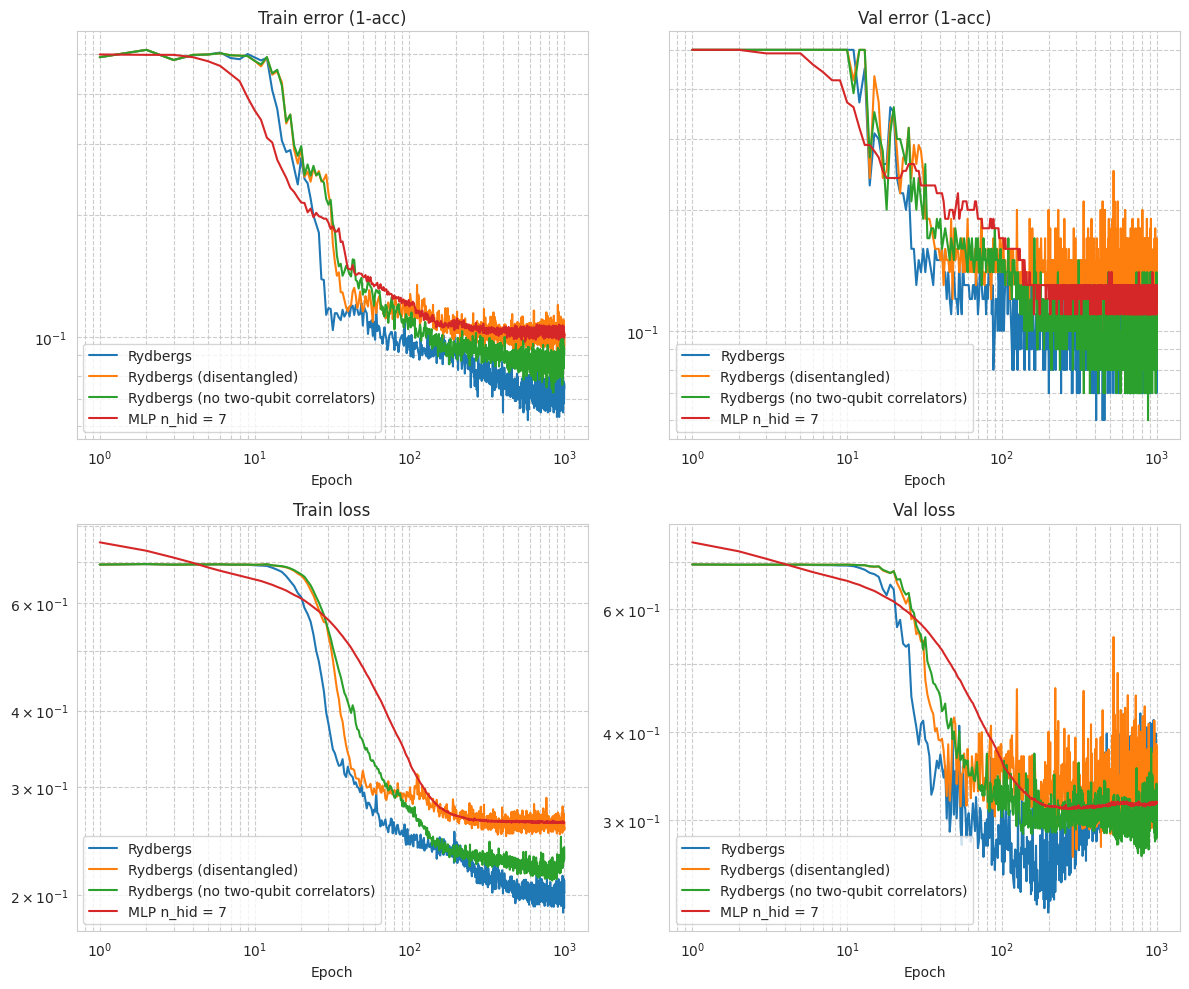
\includegraphics[width=\linewidth]{images/sklearn_results.png}
         \caption{Многомерный датасет (4 признака).}
         \label{fig:results_sklearn}
     \end{subfigure}
     \vspace{0.5cm} % Отступ между верхним и нижним графиком
     \begin{subfigure}[b]{0.8\textwidth}
         \centering
         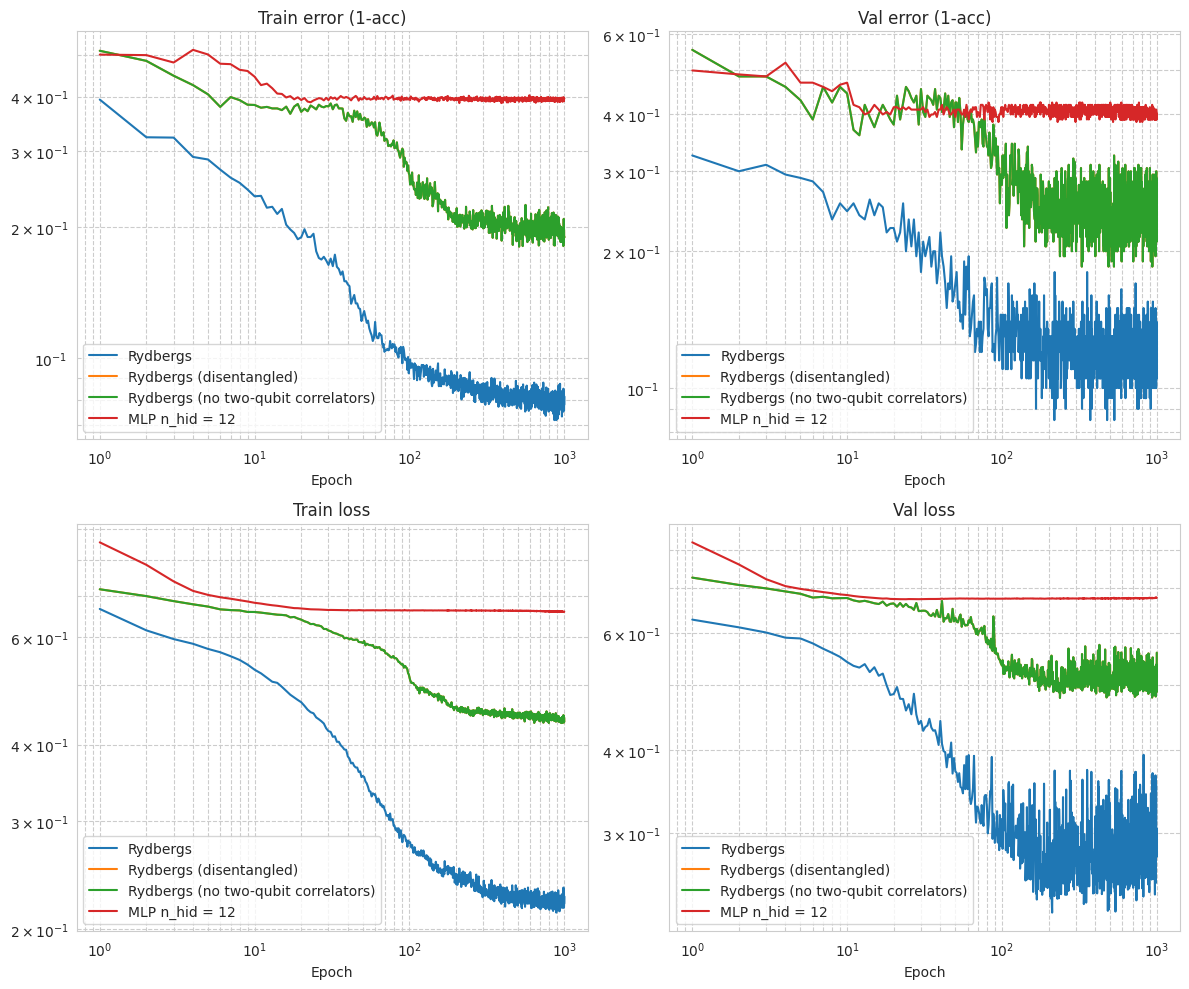
\includegraphics[width=\linewidth]{images/spiral_results.png}
         \caption{Спиральный датасет (2 признака).}
         \label{fig:results_spiral}
     \end{subfigure}
     \caption{Кривые обучения (Train/Val Error и Loss) для предложенной архитектуры на базе ридберговских атомов и классического MLP-бейзлайна. Сравнение включает полную модель, режим без межатомного взаимодействия (disentangled) и вариант без использования двухкубитных наблюдаемых.}
     \label{fig:training_curves}
\end{figure}
